\section{\system Design}
\label{sec:design}

\begin{figure}[!htbp]
\centering
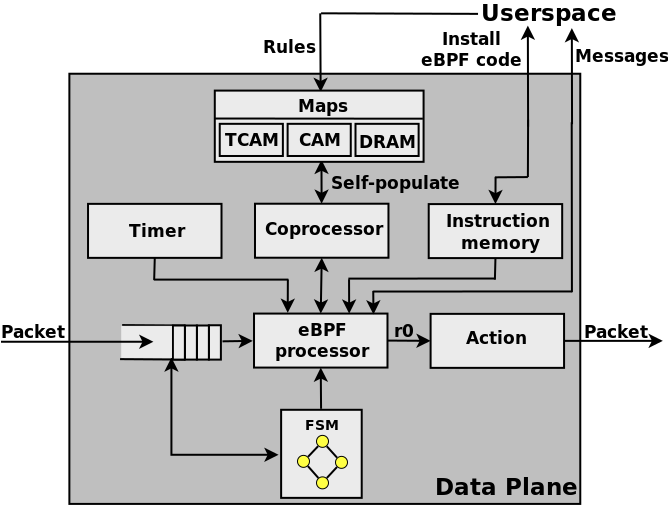
\includegraphics[width=1.\linewidth]{figures/06_fig01.png}
\caption{Packet processor datapath design and implementation on NetFPGA SUME.}
\label{fig:06_fig01}
\end{figure}

Figure~\ref{fig:06_fig01} gives an overview of the packet processor design and implementation built on top of the NetFPGA SUME~\cite{SUME2014} platform. 
Each box represents a hardware module.
%The device design is represented by the orange modules and Tables module.
They are described in Section~\ref{sec:implementation}.


\subsection{Data plane}

The packet processor extends the NetFPGA datapath with four new hardware modules: instruction memory, eBPF processor, coprocessor, and action packet. There is also a modification to the Finite State Machine (FSM) of Output Port Lookup module.
There is also new hardware modules to store eBPF maps.
The eBPF instructions generated from the user-created C and P4 codes are stored in the instruction memory. These instructions define the behavior of the data plane. The eBPF processor is responsible for performing the parse, matching, and actions using instructions stored in the instruction memory. In addition, the processor communicates with the control plane through a socket. The coprocessor handles requests to access the tables. The action module in the packet only forwards or discards the packet according to the value stored in eBPF register R0 after processing the eBPF instructions. % Further details on the implementation of the data plan are presented in the \ ac {[ref]} section.

\subsection{Metadata}
\label{sec:metadata}

% \begin{figure}[ht]
% \centering
% 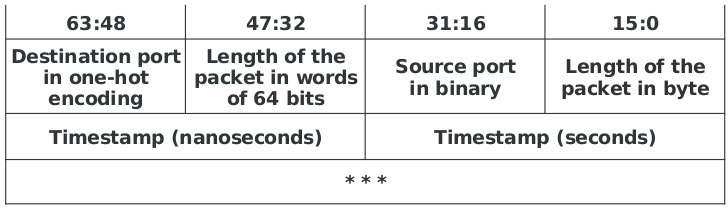
\includegraphics[width=1.\linewidth]{figures/06_fig03.png}
% \caption{Metadata: Information retrieved from the input queue about the packet that is stored in the data memory of the eBPF processor.}
% \label{fig:06_fig03}
% \end{figure}

\begin{table}[htp]
\centering
\caption{Metadata: Information retrieved from the input queue about the packet that is stored in the data memory of the eBPF processor.}
\label{tab:metadata}
\resizebox{\linewidth}{!}{%
\begin{tabular}{|c|c|c|c|c|c|c|}
\hline
\multicolumn{2}{|l}{0} &\multicolumn{3}{c}{bit} &\multicolumn{2}{r|}{255}\\
\hline
8 bits & 8 bits & 8 bits & 32 bits & 32 bits & 16 bits & 152 bits \\
\hline
Input & Source & Destination & Time-    &  Time-       & Length & Free \\
Port  & Queue  & Queue       & stamp (s)& stamp (ns)   & (bytes) & \\
\hline
\multicolumn{7}{|c|}{Ethernet Frame} \\
\hline
\multicolumn{7}{|c|}{Payload} \\
\hline
\end{tabular}}
\end{table}

% \begin{table}[ht]
% \centering
% \caption{Metadata: Information retrieved from the input queue about the packet and stored in the data memory of the eBPF processor.}
% \begin{adjustbox}{max width=.8\textwidth}
% \label{tab:metadata}
% \begin{tabular}{|c|c|c|c|}
% \hline
% 63:48 & 47:32 & 31:16 & 15:0 \\
% \hline
% \begin{tabular}[c]{@{}c@{}}Destination \\port in one-hot\\encoding \end{tabular} &
% \begin{tabular}[c]{@{}c@{}}Length of the\\packet in\\words of 64 bits\end{tabular} &
% \begin{tabular}[c]{@{}c@{}}Source port\\ in binary\end{tabular} &
% \begin{tabular}[c]{@{}c@{}}Length of \\the packet \\in bytes\end{tabular} \\
% \hline
% \multicolumn{2}{|c|}{\begin{tabular}[c]{@{}c@{}}Timestamp (nanoseconds)\end{tabular}} &
% \multicolumn{2}{|c|}{\begin{tabular}[c]{@{}c@{}}Timestamp (seconds)\end{tabular}} \\
% \hline
% \end{tabular}
% \end{adjustbox}
% \end{table}


The data plane receives the packet through the input interface and stores the packet in the input queue with some additional information called metadata.
%Figure~\ref{fig:06_fig03} shows the stored structure.
%Figure~\ref{fig:06_fig03}
Table~\ref{tab:metadata} shows the metadata header. First line indicates the byte order and size. The other lines show the stored structure.
After the metadata is received, comes the Ethernet frame. Metadata header fields can also be used by the eBPF program, as well as, any other protocol field. The currently defined metadata are the destination port, packet size in multiples of 64-bit, source port, packet size in bytes, timestamp in nano seconds and seconds. The fields of packet size, in multiples of 64-bit and bytes, are included because the input queue module already provided this information.

\subsection{Actions}

\begin{table}[ht]
\centering
\caption{Action performed on the packets.}
\label{tab:action}
\resizebox{\linewidth}{!}{%
\begin{tabular}{|c|c|l|}
\hline
\textbf{Action}   & \multicolumn{1}{c|}{\textbf{Code}} & \textbf{Description} \\ \hline
\begin{tabular}[c]{@{}c@{}}Forwarding\end{tabular}  & 0 - 0xFFEF & Forwards packet. \\ \hline
Controller     & \begin{tabular}[c]{@{}c@{}} 0xFFF3\end{tabular}                           & Send packet to the controller. \\ \hline
\begin{tabular}[c]{@{}c@{}}Drop \end{tabular}  & 0xFFF0 & Drop packet. \\ \hline
\begin{tabular}[c]{@{}c@{}}Flood \end{tabular} & \multicolumn{1}{c|}{0xFFFF}  & \begin{tabular}[c]{@{}c@{}}Send packet to all ports\\except for the input port.\end{tabular} \\ \hline
\end{tabular}}
\end{table}


The return value of the eBPF processor, which is stored in register R0, is used to determine which action should be performed with the packet. Table~\ref{tab:action} describes the return values of eBPF and their respective actions. After eBPF finishes its computation, the packet can be: forwarded to the exit port; forwarded to the controller; discarded; flooded to all ports with the exception of the input port.

%The NetFPGA hardware consists of four Ethernet ports. Each port contains one MAC and one CPU queues (Figure~\ref{fig:06_fig01}) where the packet can be routed. The coding values of the respective actions are based on the one-hot encoding of the queues.

eBPFlow enables other dynamic actions such as modifying the packet header, packet payload, adding or removing fields.
%Unlike RMT~\cite{bosshart2013forwarding}, 
Some NFs like stream cypher requires to modify the packet payload. Other NFs, like load balancer, only require to modify the packet header. The controller can configure the hardware to enable or disable modifying the packet payload. For NFs that do not require packet payload modification, this is an optimization.
Since the packet is stored in the data memory, a store instruction modifies the packet. The packet content can also be used for arithmetic and logical operations, for example, decrementing TTL or recomputing checksum.

